\chapter{Background}
\label{ch:background}
In this section, we provide background information on several subjects related to the work in this thesis. These include discussions on variational auto-encoders, normalizing flows, and a general description of \ac{NMT}. Further details about the particular \ac{NMT} architecture considered in this work are discussed in Chapter 3. % where more specific to this work are provided in chapter 3 on \ac{LVNMT} models.  



\section{Neural Machine Translation}
\label{section:neuralMT}

Statistical machine translation is a field which applies statistical methods to train computer systems that perform language translation. Historically these methods have typically involved learning word-level mappings, phrase tables, and language models to perform translation \cite{koehnSMT2010}. These components of the system are learned with statistical methods like expectation maximization by analyzing the \textit{bi-text} to extract relevant phrases and derive their likelihood under the provided bi-text.  In \ac{SMT} literature, \ac{NMT} refers specifically to training \ac{SMT} systems which incorporate neural networks as the primary model in the system. %Machine learning researchers also are actively studying \ac{NMT} systems. 

\ac{NMT} systems have achieved \ac{SOTA} results across a variety of language pairs over alternative approaches in the \ac{SMT} literature \cite{bahdanau2014NMTBYJoint,koehn2017NMT,vaswani2017attentionTransformer}. For human understanding, the goal is to correctly translate from source language $x$ (for example, English) to target language $y$ (for example, German) such that the sentence is coherent and captures the meaning of the source sentence.\footnote{There are other criteria for defining quality in translations including concepts such as adequacy, fidelity, and fluency \cite{Papineni2002BLEU,koehnSMT2010}.} Capturing the subjective quality of a translation makes defining an optimization  objective a difficult problem. Instead, similar to historical \ac{SMT}, \ac{NMT} systems learn to maximize the log-likelihood of the conditional distribution $p(y\cond{x})$: 
\begin{equation}
	max_{\theta} \log p_{\theta}(y \cond{x})  = \sum_{i=1}^{T} \log p_{\theta}(y_{i} \cond{x, y_{<i}}).
\end{equation}
Here, $\theta$ represents the parameters of the \ac{NMT} model, $y_{<i}$ refers to conditioning on all previous words excluding $i$, and $T$ is the sequence length. 

There are a variety of hyperparameter choices when building an \ac{NMT} system. One core component of many \ac{SOTA} systems are auto-regressive neural networks which condition on the previous output of the network for data which have sequential relations. One category of such networks is the \ac{RNN} in which an internal hidden representation is maintained. The hidden representation can be viewed as the network's \textit{memory} of a sequence \cite{gravessupervisedSequenceRNNbook2012}. In the above objective, this hidden state generally is interpreted as allowing the system to condition on the whole source sentence $x$ and all previous target words $y_{<i}$. Unfortunately, \ac{RNN}s can suffer from long term dependencies problems. This can lead to gradients either vanishing or exploding during the training process. Researchers have developed a number of architectures to address this problem, such as the long short term memory cells \cite{gravessupervisedSequenceRNNbook2012}.

As there are several types of \ac{RNN}s, we only describe the \ac{GRU} because it is the one used in our work \cite{cho2014GRU}. The \ac{GRU} can be viewed as a simplification of a long short term memory cell which helps mitigate the effect of gradient exploding or vanishing problem due to long sequence dependencies \cite{gravessupervisedSequenceRNNbook2012}. The network can be described with the following equations
\begin{equation}
	z_{t} = \text{sigmoid}(W_{z}[x_{t}; h_{t-1} ] ) %x_{t} + U_{z} h_{t-1} + b_{z}),
\end{equation}

\begin{equation} 
	r_{t} = \text{sigmoid}(W_{r} [x_{t}; h_{t-1}] )  \circ h_{t-1},%(W_{r} + U_{r} h_{t-1} + b_{r}) their
\end{equation}

\begin{equation}
	h_{t} = (1 - z_{t}) \circ h_{t-1} + z_{t} \circ (W_{h} [x_{t}; r_{t} ]). % \text{tanh} (W_{h}x_{t} + U_{h} (r{t} \circ h_{t-1}) + b_{h}) 
\end{equation}
In these equations, $W_{z}, W_{r}, W_{h}$ represent the learned weight matrices which can include a bias term,  $[a ; b]$ refers to a concatenation operation, and $\circ$ is the element-wise product. Intuitively, the \ac{GRU} works as a soft logic gate where the \textit{update gate $z$} controls the `relevance' of previous and current state in the memory of the network. The \textit{reset gate $r$} decides the importance of previous information in conjunction with the new input. 

Whether choosing the \ac{GRU}, or alternatives,  all \ac{NMT} models generally follow the \ac{seq2seq} framework \cite{vinyals2015grammaras}. In \ac{seq2seq} models, the source sentence $x$ is \textit{encoded} as a series of latent representations capturing words-in-context information. A \textit{decoder} utilizes these hidden states, such as for initializing its own hidden state, to help inform the decoding process for target sentences $y$. The decoder can be interpreted as a conditional \textit{neural language model} \cite{koehn2017NMT}.\footnote{This simply means a neural network is chosen to model the joint probability of a sentence $p(y_{1}, y_{2}, ..., y_{T})$ with a continuous representations.}

The one other major consideration for \ac{NMT} is picking the best translation. A naive solution is to take the most likely word at each step of decoding. This can lead to the \textit{garden-path}, or \textit{label bias}, problem in which case the most likely words at the current time step lead to a series of unlikely words later in translation \cite{lafferty2001CRF,koehn2017NMT}. Instead, typically \textit{beam search} is employed to maintain $n$ possible beams (translation hypotheses) \cite{koehn2017NMT}. At each step, after committing to the top $n$ beams  in the previous time step, a score function is calculated and the top $n$ new beams are selected. The score function is the partial probability up to the current time step $i$, $\prod^{T}_{i=1} p(x_{i} | x_{<i})$. When a beam encounters an end-of-sentence token, or designated maximum length, it is held out and the number of active beams is reduced. Once all beams are in-active, the best translation is then chosen from the remaining beams based on their probability normalized by length $\frac{p(y_{1}, ..., y_{n})}{n}$. 

\begin{figure}
	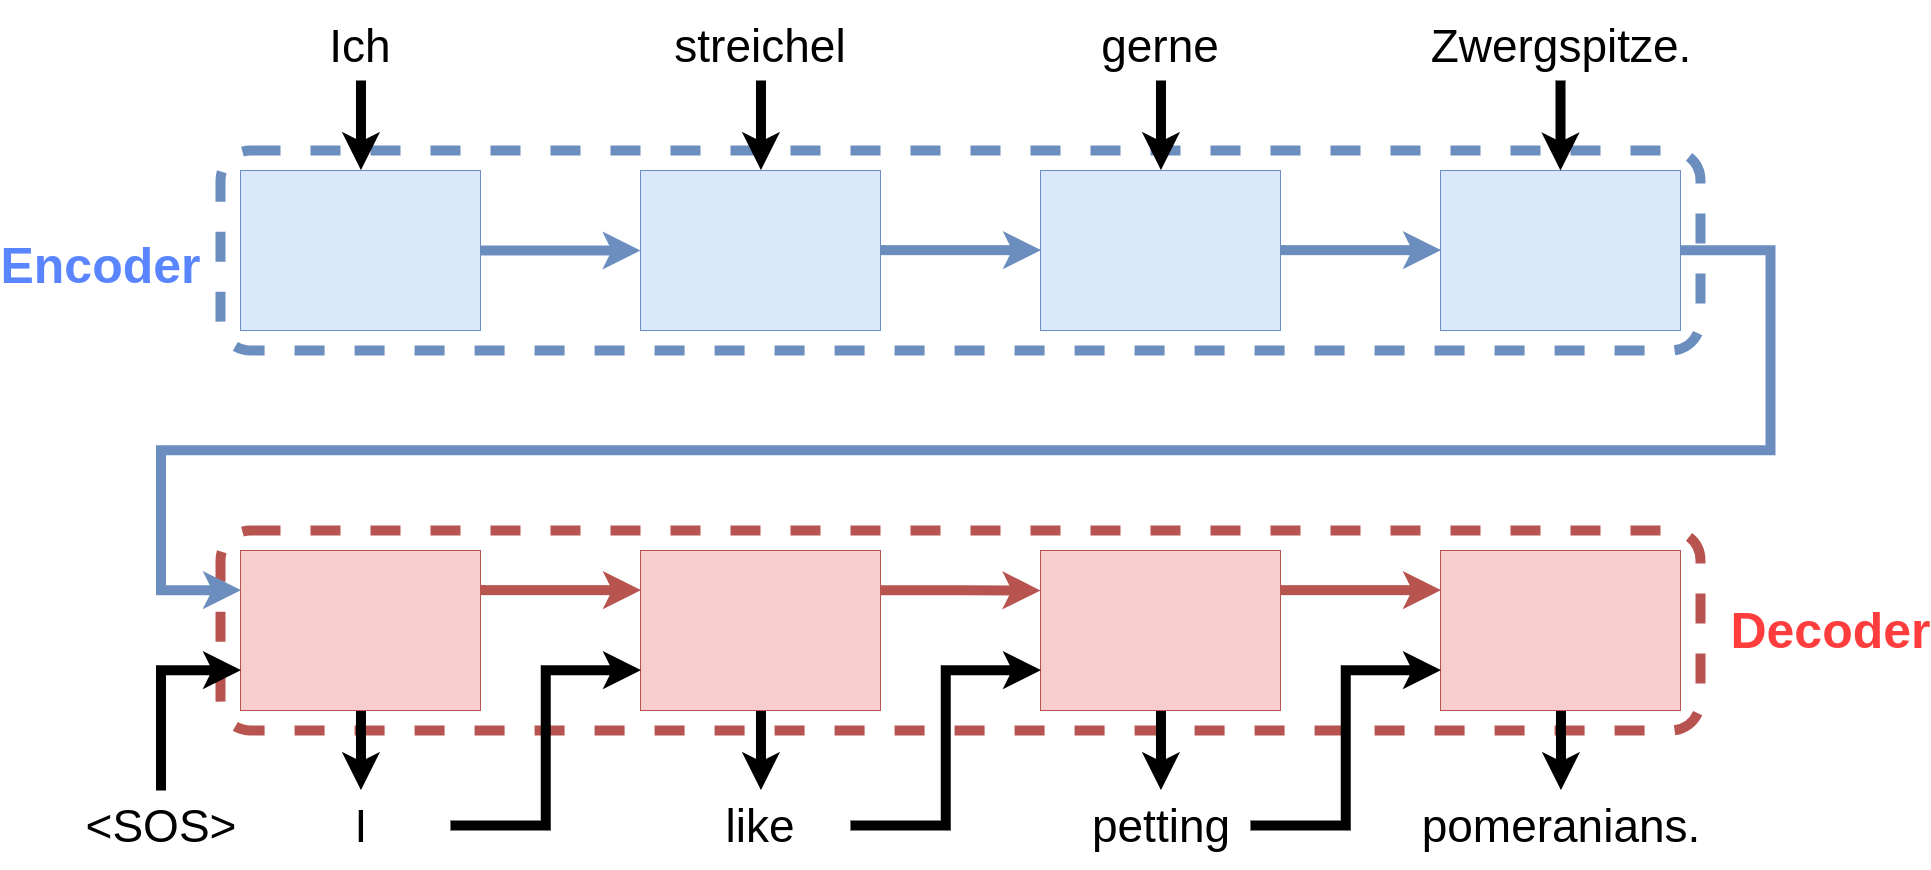
\includegraphics[width=\linewidth]{seq2seq.png}
	\caption{Simplest formulation of a \ac{seq2seq} model in \ac{NMT} \cite{sutskever2014seq2seq}.} 
	\label{fig:seqseq2}
\end{figure}



\section{Variational Autoencoders}

The \ac{VAE} is a class of generative model which represent the joint distribution $P(X, z)$, where $X$ is the data set and $z$ is an introduced random variable. The joint distribution is factorized typically as follows: $p(X, z) = p(X\cond{z})p(z)$. This is interpreted as assuming the dataset $X$ was generated by latent process  $z$. 

An important aspect of \ac{VAE}s is amortized inference, which involves introducing functions $f(x)$ that produce distribution parameters for each sentence pair in our case.\footnote{More generally, the amortization function learn distribution per datum, which could be of any modality or appropriate representation depending on the application.} The motivation for employing amortized inference is eliminating the need to learn separate distribution parameters for each sentence pair. Otherwise, each sentence pair would require their own parameters, requiring much more computation. In \ac{VAE}s this function is typically represented with a neural network. Throughout this paper when we describe any distribution as $p_{\theta}(\cdot)$, the chosen Greek symbol (as it will vary beyond $\theta$) to represent the parameters of neural networks which handle amortization of $p(\cdot)$. 

In order to learn a good representation of $p(X,z)$ the objective is to maximize the log-likelihood of the marginal distribution $p(X)$. To calculate $p(X)$ one then would need to integrate over the random variable $z$:
\begin{equation}
\log p(X) = \log \int p(X \cond{z}) p(z) dz.
\end{equation}

Unfortunately, this integral is generally considered intractable. This is often due to choosing a neural network to handle the amortization of distribution parameters. This could be addressed by Monte Carlo sampling from $p(z)$, but the latent variable is unknown and the posterior $p(z \cond{X})$ is also difficult to calculate. 

Instead, researchers often solve this problem with optimization. This involves applying \ac{VI} to learn an approximation of the true posterior $p(z \cond{X})$. This introduces a variational distribution $q_{\phi}(z \cond{X})$, parametrized by some neural network $\phi$, which will be optimized along with our model. This can be interpreted as introducing an inference network which performs the amortization of the prior parameters $p(z)$ as discussed previously. The objective in \ac{VI} then involves maximizing the \ac{ELBO}, or variational free energy, on the joint distribution $p(X, z)$ and $q(z \cond{X})$: 

\begin{equation}
	log p_{\theta}(x) \geq \E_{q_{\phi}(z \cond{X})} [ log(P_{\theta}(X \cond{z}) ]  - KL(q_{\phi}(z \cond{X}) || p(z)).
\end{equation}

An important thing to note in the above equation is that the prior $p(z)$ is typically chosen to be stationary. This means the \ac{ELBO} can be interpreted as optimizing two conflicting objectives. The expectation term seeks to maximize the reconstruction of data from $z$ whereas the second term bounds the variational distribution to stay within some latent space.

Despite this conflict we have gained some important properties. As the KL divergence is non-negative, and only 0 when the distributions match (in other words, they are identical), it is theoretically possible to recover the true log-likelihood of the data. We can also sample from $q_{\phi}(z \cond{X})$ to approximate the expectation term which was not possible before.

Unfortunately, directly sampling $q_{\phi}(z \cond{X})$ introduces a discrete operation which means we cannot calculate gradients end-to-end in the model. One approach to mitigate this is the \textit{re-parametrization trick} in which the variational distribution  is rewritten as a function and sampling is done from some surrogate  distribution \cite{kingma2014autoencodingVB,rezende2014stochasticBackprop} . Here, we show this approach for the isotropic Gaussian with mean $\mu$ and variance $\sigma$ conditioned on $x$
\begin{equation}
f_{\phi}(x, \epsilon) = \mu_{\phi}(x) + \epsilon \circ \sigma_{\phi}(x), \epsilon \sim N(0, 1).
\end{equation}

Here, $\circ$ is an element-wise operation between each dimension $\sigma_{\phi}(x)$ and $\epsilon$. With this, the expectation in the \ac{ELBO} can be rewritten with respect to $p(\epsilon)$ and enables end-to-end optimization 
\begin{equation}
\log p_{\theta}(x) \geq \E_{p(\epsilon) } [ \log(P_{\theta}(X \cond{f_{\phi}(x, \epsilon)}) ]  - KL(q_{\phi}(z \cond{X}) || p(z)).
\end{equation}





%In order to optimize this objective requires Monte Carlo integration, in which samples are drawn from the variational distribution $z ~ q(z \cond{X})$ and in whicn the derivative can be calculated. This sampling proceedures can cause issues however as it cause discontinuities in the computational graph. One approach to mitigate this is the reparameterization trick \cite{kingma2014autoencodingVB,rezende2014stochasticBackprop} in which the variational distribution  is rewritten as a function and sampling is done from some surrogate distribution. Here, we show the this approach for the Isotropic Gaussian with mean vector $\mu$ and variance $\sigma$
%\begin{equation}
%	f(\mu, \sigma, \epsilon) = \mu + \epsilon * \sigma, \epsilon \sim N(0, 1)
%\end{equation}

%With this, the expectation in the \ac{ELBO} can be rewritten with respect to the $P(\epsilon)$ and can easily be sampled from or have gradients passed through.

%\begin{equation}
%	E_{p{\epsilon} [ log P(X, z) - log q( f(\mu, \sigma, eps) \cond{X})]}
%\end{equation}

%As a means to make both the conditional distribution $P(X \cond{z})$ and $q(z \cond{X})$ computationally efficient, ammortized inference \reminder{cite something here} is employed to learn the distributions. In the regular variational inference setting, the sufficient statistics for a distribution would be learned per datum. This can be quite memory and computationally expensive, and instead these distributions are represented by functions which produce the distribution parameters. These can be any function, but typically neural networks parameterized by $\theta$ and $\phi$ are used to represent $P(X \cond{z})$ as $P_{\theta}(X \cond{z})$ and $q(z \cond{X})$ as $q_{\phi}(z \cond{X})$. This is where the name variational autoencoder comes from, as the variational distribution $q$ can be interpreted as an encoder, and conditional distribution $p$ represents the decoder as in the typical autoencoder model. 

\section{Normalizing Flows}

Normalizing flows are an application of the change of variables theorem in machine learning. They introduce a series of  $k$ invertible functions $f_{1:k}$ which transform a base distribution $p(z_{0})$ into another distribution $p(z_{k})$: 
\begin{equation}
p(z_{k}) = f_{k} \circ f_{k-1} \circ ... \circ f_{0}(p(z_{0})).
\end{equation} 
Here, $\circ$ is shorthand for the nested calls for functions $f_{i}$. This allows one to transform samples from the base distribution $z_{0}$ into samples $z_{k}$
\begin{equation}
	z_{K} = q_{0}(z_{0}) \prod_{k=1}^{K} \bigg|det \bigg(\frac{\delta f_{i}}{\delta z_{i-1}}\bigg) \bigg|.
\end{equation}
Alternatively, it becomes possible to do density estimation of samples by calling the inverse $f_{i}^{-1}$ on samples $z_{k}$. To our knowledge, there are 2 main ways normalizing flow models are optimized in the literature. 

%There are a number of utilities of normalizing flows which generally involve enriching the posterior distribution. In the \ac{VI} setting this translates to enabling the variational distribution $q$ to capture possible posterior representations beyond those in those achievable with the base distribution. Alternatively, it becomes possible to directly optimize the log-likelihood of the data distribution without the \ac{ELBO} with normalizing flows. 

%\begin{equation}
%	logP(z_{k}) = log(P(z_{0})) - \sum_{i=1}^{k} log |det (\frac{\delta f_{i}}{\delta z_{i-1}}) |
%\end{equation}


The first approach incorporates normalizing flows into the \ac{ELBO} which introduces an expectation term of the log absolute Jacobian with respect to the variational distribution, as follows:

\begin{equation}
\E_{q_{\phi}(z_{0} \cond{X})} [ log(p_{\theta}(X \cond{z}) ]  - KL(q_{\phi}(z_{0} \cond{X}) || p(z_{k})) + E_{q_{\phi}(z_{0}\cond{X})}\bigg[\sum_{i=1}^{k}log \bigg|\frac{\delta f_{i}}{\delta z_{i-1}}\bigg|\bigg].
\end{equation}
Previous works typically employ hyper-networks \cite{ha2016hypernets} to amortize the parameters of the normalizing flows instead of directly optimizing them  \cite{rezende2015VIwithNF,tomczak2016Householder,vdberg2018sylvester}. In the \ac{VI} setting this enables the variational distribution $q$ to capture possible posterior representations beyond those achievable with the base distribution.

Alternatively, normalizing flows enable direct optimization of the log probability of the data distribution:
 
\begin{equation}
	\log p(x) = \log p(z_{0}) - \sum_{i=1}^{k} \log \bigg| \frac{\delta f_{i}}{\delta z_{i-1}} \bigg|
\end{equation}
This approach is quite useful as it eliminates the need for the variational distribution in \ac{VI}. The choice of flow becomes particularly important though because of the dependence on the absolute log Jacobian. %some flows can be quite slow to do density estimation in order to transform the data distribution samples back to the base distribution. 

The predominant focus of normalizing flows research has been on defining invertible functions which have computationally efficient Jacobians. This has lead to a variety of flows with different Jacobian formulations such as autoregressive flows which lead to triangular Jacobians \cite{kingma2016IAF, papamakarios2017MAF}; flows which by construction have analytic Jacobians \cite{rezende2015VIwithNF,vdberg2018sylvester}, or volume preserving flows which have the Jacobian equal to one \cite{tomczak2016Householder,tran2019discreteflows,hoogeboom2019IntegerDiscreteFlows}. Note that these groupings do not necessarily reflect the full range of approaches to normalizing flows.



%\subsection{Types of Normalizing Flows}

%There are several different types of flows models. We discuss several classes of these models, but note to the reader that this does not represent an exhaustive list of existing flows models as normalizing flows are an active area of research and alternative groups may exist. 

%\subsubsection{Autoregressive Models}
%Autoregressive Flows models are models that structure the transformations such that a diagonal Jacobina matrix can be constructed. This formulation means the determinant can be calculated linearly as the determinant of diagonal matrices is just the product of the diagonal terms $\prod_{0}^{n} \sigma_{i}$. This is accomplished by making each dimension of the transformed distribution $z$ depend on the subsequent entries.



%\begin{equation}
%	 z_{i} = a + b * z_{i-1}		
%\end{equation}

%\subsubsection{Non-volume Presevering Flow Models} 
%These are models that can be shown to have the determinant equal to one. 

%\subsection{Ordinary Differential Equation Flows}

%I'm not as familiar with these, but basically your flows is an ordinary differential equation. 

%\subsubsection{Analytically Formulated Determinant Flow Models}
%This is our own classification, but several otherwise "unclassified" flows models follow this formulation. In these types of Normalizing flows,







